\chapter{绪论}\label{chapter01}
{\em 首先,本章介绍研究背景,分析保障系统正确的重要性,并阐述研究意义。其次,综合分析遗忘理论、最强必要(最弱充分)条件等关键技术的国内外研究动态,以及遗忘理论在形式化验证中的应用研究趋势。然后,围绕研究对象凝练出关键问题与目标。进一步,介绍本文的核心研究内容以及取得的主要成果。最后,给出具体章节组织安排。}
\section{研究背景与意义}
\subsection{研究背景}

形式化验证是一种广泛应用在硬件\cite{lam2007,lv2000,jani2007Verilog}和软件系统中\cite{yuan2008,gu2005}有别于测试的、采用数学方法证明系统满足给定特性的验证(verification)技术。软件和硬件系统的缺陷会导致严重的后果,如表\ref{tab:systemEvents_1.1}中列出的几个重大事件。近年来,为了减少系统(尤其是像火箭发射系统和卫星发射系统等关键领域的系统)错误带来的损失,形式化方法的研究与应用越来越受到人们的重视。INTEL、AMD、IBM、NVIDIA、CADENCE、 Motorola、西门子和微软等大型公司纷纷引入了形式化验证方法。与此同时,学术界也在形式化验证领域取得了突破性的成果,比如:剑桥大学对ARM6处理器进行了验证\cite{DBLP:conf/tphol/Fox03}, 为类似于ARM这样的处理器提供了潜在的形式化验证方法,德国的Verisoft项目验证了一个一万行的操作系统内核\cite{DBLP:conf/sefm/DaumSS09}。

\begin{table}[htbp]
\caption{由系统故障引起的重大事件概览}
\label{tab:systemEvents_1.1}
\centering
\fontsize{10pt}{\baselineskip}\selectfont
\begin{tabular}{p{0.12\textwidth}p{0.35\textwidth}p{0.35\textwidth}}%
	\toprule
	\textbf{时间}&\textbf{事故原因}&\textbf{损失}\\
	\midrule
    1991年 & 美国爱国者导弹系统舍入错误 & 28名士兵死亡、100人受伤等\\
	1996年 & 阿丽亚娜5型运载火箭软件在不同飞行条件下的代码重用 & 火箭与其它卫星毁灭\\
	1999年 & 火星探测器用错度量单位 & 探测器坠毁并造成了3.27亿美元的损失\\
	2011年 & 温州7.23动车信号设备在设计上存在严重的缺陷 &动车脱节脱轨、多人失去生命\\
	
\bottomrule
\end{tabular}
\end{table}

反应式系统(reactive system)是一种特殊的应用系统,它不终止且与环境有着持续不断的交互。
其应用十分广泛:上至航空电子等安全攸关的领域,下至生活息息相关的汽车电子。
必须在指定时间期限内完成对外部事件的检测和目标事件的响应,是安全攸关反应式系统的核心要求。
因而,近年来包括形式化方法在内的多种方法用于确保反应式系的正确性。


形式化验证有两种主要的验证方法:自动定理证明(automated theorem proving)和模型检测(model checking)。
在自动定理证明中,系统模型和规范(specification)被同一种形式化语言分别描述为$\varphi_{imp}$和$\varphi_{spec}$,然后证明其推理“$\varphi_{imp}\rto \varphi_{spec}$”或“$\varphi_{imp}\lrto\varphi_{spec}$”的正确性,即:证明模型系统$\varphi_{imp}$是否满足给定的规范$\varphi_{spec}$。
常用的自动定理证明方式有归结(resolution)\cite{DBLP:journals/jacm/Robinson65}和常用于模态逻辑的基于表推理(tableau)\cite{hughes1996new}的方法。
计算机程序和系统验证(verification of computer programs and systems)是自动定理证明的新领域,它使用基于规则的方法来验证程序的正确性。
然而,当程序为循环语句时,验证所需要的不变式(invariant)获取是个困难的问题。
%然而,在自动定理证明中寻找不变式(invariant)是一个相当困难的问题。
因此,为了避免类似于在Hoare逻辑\cite{Hoare1969}、动态逻辑\cite{harel1979first}和分离逻辑\cite{DBLP:conf/lics/Reynolds02}形式化验证过程中寻找不变式问题,Fangzhen Lin提出将一个程序(program)转换为一阶理论,
然后再使用一阶理论中的自动定理证明方法来验证\cite{DBLP:journals/ai/Lin16}。

形式化验证的模型检测首先由Clarke提出,并用于解决并发系统验证问题\cite{DBLP:conf/spin/Clarke08}。Clarke和Emerson指出,在有限状态的并发系统中,使用时态逻辑推演系统(deductive system)中的公理和推理规则进行构造性证明(proof construction)的方法证明系统是否满足给定的规范是不必要的\cite{clarke1981design}。因为在有限状态并发系统中,并发系统可以被抽象为一个Kripke结构$\Hm$,规范被表示成一个逻辑公式$\varphi$;此时,该验证问题就变成检验一个Kripke结构是否满足该公式,即模型检测($\Hm\models^? \varphi$): 判断$\Hm$是否是$\varphi$的一个模型。

近年来,模型检测问题在知识表示与推理(KR)领域的推进下取得了丰富的科研成果,例如:基于SAT的有界(bounded)模型检测\cite{DBLP:journals/ac/BiereCCSZ03}和基于OBDD的符号模型检测\cite{burch1992symbolic}已经使得模型检测问题在时间和空间效率上取得了很大的进步,在一定程度上缓解了其固有的状态空间爆炸问题。与此同时,大量优质的模型验证器,如:NuSMV\footnote{http://nusmv.fbk.eu/}、SPIN\footnote{http://spinroot.com/spin/whatispin.html}、Uppaal\footnote{http://www.uppaal.org/} 等,也相继发展起来,并且大部分的验证器都可以用来验证多种时态逻辑描述的公式。  

       
时序逻辑(也叫时态逻辑)作为一种描述系统规范的形式化语言,其研究状态随时间变化的系统的逻辑特性。由于软件和硬件系统运行的本质是状态变化的过程,所以时态逻辑在软件和硬件系统验证中应用得相当广泛。计算树逻辑(computation tree logic, \CTL)是分支时态逻辑的一种,其模型检测是多项式时间可完成的。然而,$\CTL$表达系统性质的能力不如$\mu$-演算($\mu$-calculus),如:“某给定的系统中存在一条路径,且这条路径上处于偶数位置的状态满足特定的性质”这一规范是不能用$\CTL$来表示的\cite{DBLP:series/txtcs/Schneider04}。充分考虑这两种逻辑语言自身的特性,本文主要研究$\CTL$和$\mu$-演算。因此,本文所说的公式指$\CTL$(或$\mu$-演算)公式,即用来描述一个规范(或性质)的公式是$\CTL$(或$\mu$-演算)公式。

在模型检测中,反应式系统通常用Kripe结构表示~\cite{DBLP:journals/fcsc/ZhuWXX10,DBLP:series/txtcs/Schneider04}。
当给定了反应式系统的Kripke结构模型$\Hm$和规范$\varphi$,
%在实际应用中,
就存在模型检测问题$\Hm\models^? \varphi$:
\[\hbox{系统输出=}
\left\{
\begin{array}{ll}
	Yes, \ \ \qquad \qquad  \hbox{若$\Hm\models \varphi$;} \\
	No\hbox{和负例}, \ \ \ \quad \ \ \hbox{否则。}
\end{array}
\right.
\]
%若$\Hm$满足$\varphi$,一般的验证器都会返回“yes”以表示满足;若$\Hm$不满足$\varphi$,验证器会给出一个使得$\varphi$不被$\Hm$满足的负例。
当$\Hm$不满足$\varphi$时,\emph{使用什么信息对$\Hm$进行修正,使得其满足给定的规范$\varphi$是一个重要的问题}。
这就是寻找{\em 最弱前件}(weakest precondition,WP)问题\cite{DBLP:journals/cacm/Dijkstra75},在人工智能(artificial intelligence,AI)中也称为{\em 最弱充分条件}(weakest  sufficient condition,WSC),与之对偶的另一个概念是最强必要条件(strongest necessary condition,SNC)\cite{DBLP:journals/ai/Lin01,DBLP:journals/jair/Lin03}。
%{\em 然而现有方法不能计算使得像反应式系统这类不终止系统满足给定规范的WSC。因而}

从知识抽取(或“消除”)的角度来看。出于安全考虑,查看信息时需要将有的信息隐藏而只抽取部分信息。
此外,随着时间推移,由于系统的部分信息会因某些原因而过时,需要将这样的信息在不影响其它信息的情况下“消除”。
如下示例:
\begin{example}[汽车制造企业模型]\label{car_manufacturing}
	一个汽车制造企业能够生产两种汽车:小轿车($se$)和跑车($sp$)。每隔一段时间,该企业都会做一个生产决策($d$),即:合理的生产计划。
	刚开始的时候,该企业做出了具有三个选择($s$)的方案:
	\begin{itemize}
		\item[(1)] 先生产足够的$se$,然后在再生产$sp$;
		\item[(2)] 先生产足够的$sp$,然后再生产$se$;
		\item[(3)] 同时生产$se$和$sp$。
	\end{itemize}
	这一过程可以由图~\ref{BVM}中的Kripke结构(带标签的状态转换图)$\Hm=(S,R,L)$形式化地展现出来,其中:
	\begin{itemize}
		\item $V=\{d,s, se, sp\}$为该工厂所需要考虑的原子命题集;
		\item $S=\{s_0,s_1,s_2,s_3,s_4\}$为状态空间;
		\item $R = \{(s_0, s_1), (s_1,s_2), (s_1,s_3), (s_1,s_4), (s_2,s_0), (s_3,s_0),(s_4,s_0)\}$为状态转换关系集;
		\item $L: S \rto 2^V$为标签函数,具体地:$L(s_0) = \{d\}$、$L(s_1) = \{s\}$、 $L(s_2)=\{se\}$、 $L(s_3) = \{sp\}$和$L(s_4) = \{se,sp\}$。
	\end{itemize}
	\begin{figure*}[ht]
		\centering
		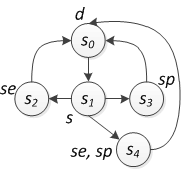
\includegraphics[width=4cm]{NnewCar.png}\\
		\caption{汽车制造企业模型}\label{BVM}
	\end{figure*}

假定,由于经济危机或者战略调整,导致该企业不能再生产跑车。这意味着所有规范和Kripke结构都不再需要考虑$sp$的,因此应该“移除”。
\end{example}

日常生活中也有很多上述例子中的场景,如:商业交易过程、软件开发过程等~\cite{Baier:PMC:2008}。
但是对于给定原子命题集,\emph{从这些大型系统(或规范)中“移除”一些原子命题,而保留与这些原子命题无关的性质是一个复杂的问题}。
%此外,在这种情形下,两个重要的概念:最强必要条件(SNC)和最弱充分条件(WSC)问题也随之产生,其中SNC是指最一般的结论,WSC指最特殊的诱因。

%基于上述存在的问题,下面给出一些解决方案及其意义所在。


\subsection{研究意义}
最强后件(the strongest post-condition,SP)和最弱前件(WP)(分别对应于上文提到的SNC和WSC)是形式化验证中两个重要的概念,其不仅被用于汇编语言程序推理~\cite{legato2002weakest}和制定验证条件\cite{DBLP:journals/ipl/Leino05},还被应用于形式化验证过程中的负例生成\cite{dailler2018instrumenting}和系统精化(refinement)\cite{woodcock1990refinement}。
当模型$\Hm$不满足规范$\varphi$($\Hm\not \models \varphi$)时,找到某个性质$\psi$,使得若$\Hm$按照此性质进行修改后得到的新模型$\Hm'$能满足$\varphi$是必要的,即$\psi$是使得$\Hm\models \varphi$成立的充分条件($\Hm \models \psi\rto \varphi$)。
然而,现有方法不能直接应用于如下情形:计算当$\Hm$为不终止系统(如:反应式系统)时使得“$\Hm\models \varphi$”为真的最强必要条件和最弱充分条件
(其详细原因将在下文指出)。此时,\emph{探索如何计算“在$\Hm$下,使得$\varphi$满足的定义在某个符号集合上的SNC和WSC”将更进一步完善模型检测问题,
同时也为基于WSC的负例生成和精化提供了理论依据和新的计算方法。}

本文将探索一种称为\emph{遗忘}(forgetting)的方法来计算充分(必要)条件。如下问所说,遗忘理论作为知识表示与推理(KR)中的重要理论,具有较长的科研历史,且在许多逻辑中都有了较为成熟的研究。然而,在时序逻辑方面的研究目前还不成熟。因此,\emph{本文的研究将为时序逻辑下遗忘理论的研究提供一个理论框架。
与此同时,借助遗忘计算上述形式化验证问题中的充分(必要)条件,架起了KR与形式化验证的桥梁。}

\section{相关研究工作回顾}
\emph{遗忘}是一种重要的知识抽取工具,它具有均匀插值(uniform interpolation)和二阶量化消解(second-order quantifier elimination,SOQE)两种称谓。
在很长一段时间内,遗忘被用于描述逻辑中本体(ontology)摘要的提取、敏感信息的隐藏和软件工程中计算两个文件的逻辑差(logical differences)。此外,其也被用于包括信念更新(belief update)、修改(repair)、规划(planning)和知识独立性的其它领域。

{\em 反应式系统}是一种不终止的、与环境有着持续不断交互的系统,其应用广泛、种类繁多。本文探究如何使用遗忘计算反应式系统下的SNC(WSC),下面就与本文密切相关的反应式系统、遗忘理论和SNC(WSC)进行回顾。

%在规划中,遗忘主要用来计算其对应的后继状态公里所需要的SNC和WSC。下面就与本文密切相关的遗忘理论和SNC(WSC)进行详细的回顾。


\subsection{反应式系统}
随着应用程序在各个领域的应用,对其需求已经发生了重大变化,继而引起模式变化。
以前,一个大型应用程序的运行通常需要数十台服务器,这么高昂的代价换来的是效果和维护成本不成正比:秒级的响应时间,需要数小时的维护。
当前,移动和云端技术的成熟使应用程序不拘泥于以前的方式,它们可以被部署到移动设备和具有多核心处理器的云端集群上。
但是,用户对应用程序的响应时间要求从秒级变到毫秒级,相应的成功率要求为100\%;程序需要处理的数据量也从之前的GB级扩展到现在的PB级。
原有的软件架构已经无法满足当前的需求。

在这种背景下,应用程序需要具备以下特质:即时响应性(Responsive)、回弹性(Resilient)、弹性(Elastic)以及消息驱动(Message Driven)\footnote{https://www.reactivemanifesto.org/zh-CN}。
反应式系统是一种与环境有着持续不断交互的系统,具有不终止的性质~\cite{DBLP:series/txtcs/Schneider04}。此外,其同时满足上述几种要求,且从传统的静态模式逐步向动态、开放、自适应、服务化的模式演化~\cite{jian2012}。
反应式系统由来已久~\cite{DBLP:conf/nato/HarelP84,DBLP:books/sp/trends86/Pnueli86},且种类繁多,如微处理器(microprocessor)、计算机操作系统(computer operating systems),航空交通管制系统(air traffic control systems)、车载电子设备(on-board avionics)以及其它嵌入式系统。

此外,反应式系统的应用非常广泛:包括航空电子等安全攸关的领域和生活息息相关的汽车电子等领域。
安全攸关反应式系统的核心要求是:必须在指定时间期限内完成对外部事件的检测和目标事件的响应,否则会产生灾难性的后果~\cite{wangjuan2019}。
为了确保反应式系统的正确性和实时性,研究者们提出了不同的解决方法,包括:模型检测方法~\cite{DBLP:books/daglib/0007403,clarke1996model,DBLP:series/txtcs/Schneider04}、目标驱动的运行时需求建模框架~\cite{jian2012}、基于图模型的实时规则调度方法(graph-based real-time rule scheduling,简称GBRRS)~\cite{wangjuan2019}、SPARDL~\cite{wangzhen2012}和选择性测试方法~\cite{lishu2004}等。
%这些应用的核心为嵌入式周期控制系统(一种反应式系统),该系统的行为不仅与自身的定义和状态有关,还与控制软件所处的环境有关。
%\begin{itemize}
%	\item 即时响应性:只要有可能, 系统就会及时地做出响应。
%\end{itemize}

在上面的方法中,多数是验证(检测)给定的系统是否具有某种性质。而当系统不满足该性质时,对如何寻找可靠的信息(称为充分条件)来对系统进行修改至关重要。
反应式系统是一种不终止的系统,通常被看作一个Kripke结构。基于此,本文探索如何计算该充分条件,使得系统在该条件下满足给定的性质。




\subsection{遗忘理论}\label{chapter01:forgetting}
遗忘这一词源于Lin等人关于一阶逻辑(first-order logic, FOL)的工作~\cite{lin1994forget},在此之前的研究中多提到的是均匀插值~\cite{visser1996uniform,konev2009forgetting}和SOQE~\cite{ackermann1935untersuchungen}。

在命题逻辑中(propositional logic,PL),公式$\varphi$遗忘一个原子命题$p$,通常记为$\Forget(\varphi,\{p\})$,得到的结果为$\varphi[p/\bot] \vee \varphi[p/\top]$(其与$\exists p\varphi$等价),其中$\varphi[X/Y]$为将$\varphi$ 中 $X$的全部出现替换为$Y$得到的结果。
%在Lin等人的文章中也将$\varphi[p/\bot] \vee \varphi[p/\top]$用$\exists p\varphi$来表示~\cite{lin1994forget}。
公式$\varphi$中遗忘有限原子命题集$P$的定义如下:
\begin{alignat*}{2}
	&  \Forget(\varphi, \emptyset) = \varphi, \qquad \\ % \nonumber
	&  \Forget(\varphi, P \cup \{q\})  = \Forget(\Forget(\varphi, \{q\}), P).
	\nonumber
\end{alignat*}

在FOL中,遗忘通常被看作SOQE问题的一个实例:从FOL公式$\varphi$中遗忘一个$n$-元谓词$P$,得到的结果为一个二阶公式$\exists R \varphi[P/R]$~\cite{lin1994forget},其中$R$为$n$-元变量。
从这个角度看来,遗忘就是找到一个与二阶公式$\exists R \varphi[P/R]$等价的一阶公式。
然而,二阶逻辑的表达能力严格大于一阶逻辑,因而可以容易得出FOL下的遗忘不是封闭(存在)的结论,也就是从某些一阶公式中遗忘某些谓词得到的结果不可以用一阶公式来表示。
作为FOL的一个子类,描述逻辑公式的遗忘也不总是存在的~\cite{DBLP:journals/ai/KonevL0W13},甚至对最基本的描述逻辑{\cal ALC}而言,遗忘的存在性问题都是不可判定的。
尽管如此,描述逻辑作为一种在语义网领域很重要的语言,其子类中的遗忘通常被用来抽取视图(review)~\cite{Wang:AMAI:2010,DBLP:conf/ijcai/LutzW11,Konev:JAIR:2012,DBLP:conf/ijcai/ZhaoS17,DBLP:conf/aaai/ZhaoSWZF20}。这些子类包括:ALCOI(the basic ALC extended with nominals and inverse roles)和ALCOIH(ALCOI extended with role hierarchies, the universal role and role conjunction)。%textcolor{red}{(包括{\cal ALCOHI}和{\cal ALCOIH})}

现有计算一阶逻辑和描述逻辑遗忘的方法有基于归结和基于Ackerm- ann引理的方法~\cite{DBLP:books/daglib/0023036}。
其中基于归结的方法是一种基于子句归结的方法,其基础是归结规则。通常在这种方法中首先把公式转换为其子句形式,然后使用归结规则,最后移除含有要遗忘的谓词(原子命题)的子句,得到的结果可能就为遗忘的结果(在后文中会详细介绍与本文相关的归结规则和转换规则)。
基于Ackermman引理的方法主要是直接或间接(扩展)使用下面的Ackermann引理得到的。
\begin{lemma}[引理 6.1~\cite{DBLP:books/daglib/0023036}]
	给定关系变元$X$和一阶公式$\alpha(\overline{x}, \overline{z})$和$\beta(X)$,其中$\overline{x}$和$\overline{z}$为普通变元构成的多元组、$\overline{x}$中变元的个数与$X$的参数个数相同、且$\alpha$中不包括$X$。
	\begin{itemize}
		\item 若$\beta(X)$关于$X$是正的,即:$X$在$\beta(X)$中的每次出现前面都有偶数个“$\neg$”符号,则:
		$$\exists X \{\forall \overline{x} [X(\overline{x}) \rto \alpha(\overline{x},\overline{z})] \wedge \beta(X)\} \equiv \beta(X)_{\alpha(\overline{x},\overline{z})}^{X(\overline{x})}\hbox{。}$$
		\item 若$\beta(X)$关于$X$是负的,即:$X$在$\beta(X)$中的每次出现前面都有奇数个“$\neg$”符号,则:
		$$\exists X \{\forall \overline{x} [ \alpha(\overline{x},\overline{z}) \rto X(\overline{x})] \wedge \beta(X)\} \equiv \beta(X)_{\alpha(\overline{x},\overline{z})}^{X(\overline{x})}\hbox{。}$$
	\end{itemize}
其中,$\beta(X)_{\alpha(\overline{x},\overline{z})}^{X(\overline{x})}$表示将$\beta(X)$中$X(\overline{x})$的全部出现用$\alpha(\overline{x},\overline{z})$来替换得到的公式。
\end{lemma}



\emph{知识遗忘}(knowledge forgetting)在模态逻辑S5中首先被提出并被用于推理智能体的知识状态(知识或者信念)~\cite{Yan:AIJ:2009}。
因为模态逻辑系统中引入了模态词,模态逻辑中的遗忘不同于经典逻辑下的遗忘。所以,不能以简单的谓词(命题)替换的方式获取遗忘的结果,如:
\begin{example}\cite{Zhang2008Properties}
	令S5公式$\varphi=\MPK p \wedge \neg \MPK q \wedge \neg \MPK \neg q$,则使用命题逻辑下的计算方法得到的结果为$\varphi[q/\top] \vee \varphi[q/\bot] \equiv \bot$。
	这显然是不正确的,因为在遗忘$q$之后智能体的知识库不应该变得不一致。
\end{example}
为此,新的计算方法和四个能精确描述知识遗忘的基本公设被给出,这几个公设为:削弱(weaking)、正支持(positive persistence)、负支持(negative persistence)和无关性(irrelevance)。
%值得注意的是这四个条件与知识遗忘形成了“当且仅当”的关系。换句话说,当知道某一个公式满足那四个条件则该公式为遗忘的结果,当知道某一结果为遗忘结果时它一定满足那四个基本条件。
此外,模态谓词逻辑下信息不完备的知识遗忘~\cite{wenximing2019buwanbei}、模态一阶逻辑S5中的遗忘也得到了研究~\cite{Yongmei:IJCAI:2011},Fang等人讨论了关于多模态(multi-modal)$K_n$、 $D_n$、 $T_n$、$K45_n$、 $KD45_n$情形下遗忘的存在性~\cite{DBLP:journals/ai/FangLD19,wenximing2019,wenximing2019kn}——这些逻辑里的遗忘总是存在的,其中$n$为智能体的个数。


均匀插值作为遗忘的一个对偶概念。
从形式上说,如果一个逻辑系统${\cal L}$中任意的公式$\varphi$和$\psi$,若$\varphi\models_{\cal L} \psi$,则存在一个公式$\xi$使得$\varphi\vdash_{\cal L}\xi$、$\xi\vdash_{\cal L}\psi$和 $\Var(\xi)\subseteq \Var(\varphi)\cap \Var(\psi)$,
则${\cal L}$具有或Craig插值性质,若$\xi$与$\psi$无关,则${\cal L}$具有均匀插值性质。

其在模态逻辑和时序逻辑系统中取得了一系列研究成果:LTL、$\CTL$和$\CTL^*$不具有均匀插值性质~\cite{Maksimova:JANCL:1991,DAgostino:synthese:2008},
S5、K和KD模态逻辑系统具有均匀插值性质~\cite{DBLP:journals/aml/Iemhoff19},
而一些模态逻辑系统没有均匀插值性质。如:量词模态逻辑S5(quantified modal logic S5)\cite{DBLP:journals/jsyml/Fine79}、K4、和S4及其扩展都没有均匀插值性质~\cite{DBLP:journals/ndjfl/Schumm86},因而其遗忘也不是封闭的。
研究具有均匀插值性质的模态逻辑遗忘可以借鉴S5系统的遗忘方法,也可以参考K系统下基于归结计算均匀插值的方法。
对于那些没有均匀插值的模态逻辑系统,可以考虑模态逻辑下的Ackermann引理~\cite{DBLP:books/daglib/0023036}。



%此外,Feng等人也研究了S5下如

在非单调推理(non-monotonic reasoning)环境中,科研工作者们也从遗忘需要满足的基本条件的视角研究了
基于回答集语义的逻辑程序的遗忘,这些工作包括Zhang、Wang等人发表在AI、AAAI和JAIR上的文章~\cite{DBLP:Zhang:AIJ2006,DBLP:journals/ai/EiterW08,Wong:PhD:Thesis,DBLP:journals/jair/WangZZZ14,wang2013forgetting,DBLP:conf/aaai/WangWWZ15,DBLP:journals/jair/Delgrande17,gonccalves2020limits},和Eiter、Gonccalves等人的综述~\cite{eiter2019brief,gonccalves2021forgetting}。


%应用
遗忘有很多应用,这里列出下面几点:
\begin{itemize}
	\item 计算后继状态公理:在规划问题中,根据最强必要条件和最弱充分条件有利于求出后继状态公理\cite{DBLP:journals/jair/Lin03}。%在该文章中,最强必要条件和最弱充分条件都用遗忘来计算;
	\item 信息隐藏:在某些关键领域,为实现隐私保护,必须隐藏敏感信息。现有方法包括基于本体\cite{DBLP:journals/ai/KonevL0W13}和基于DataSecOps的个人信息保护\cite{wangwen2021}。要做到隐私保护,只需要隐藏(遗忘)那些敏感的概念(concept)和角色(role)符号。值得注意的是,个人信息保护涉及被遗忘权\cite{zhujia2020};
%	\item 计算逻辑差:
	\item 知识更新:在许多场景,知识不是一层不变的,随着时间或空间的推移,会有新的知识加入。如何用新加入的信息更新原有知识,而保证知识库的一致性是知识更新需要解决的问题。此外,知识更新也需要满足一些基本条件。在这些基本条件中,Katsuno和Mendelzon提出的$(U1)$-$(U8)$较为常用;%,本文也使用这几个基本条件;
	\item 提取本体的概要:当一个本体工程师想要快速了解并测试一个本体的内容时,能事先快速地摒弃许多无关信息,并提取出本体的概要是非常有用的;
	\item 知识归并:知识库通常来自于多个信息源,这些分布的信息大多会存在冲突(不一致),因而不能简单地将它们放在一起。归并考虑当这些信息矛盾时如何将它们整合\cite{DBLP:journals/tkde/LiberatoreS98,DBLP:journals/logcom/KoniecznyP02,DBLP:journals/jair/Maynard-ZhangL03,konieczny2004da2,DBLP:journals/ai/EveraereKM10},且基于遗忘的归并可以尽可能少地遗忘原子以保持知识的一致性\cite{xudai2011}。
	\item 逻辑独立性:生活中许多场景都需要判断哪些信息是无关的(或相关的),即信息的独立性\cite{DBLP:journals/jphil/Sandu93,DBLP:journals/igpl/Sandu97,DBLP:journals/igpl/Vaananen02,DBLP:journals/synthese/Sevenster06},如:知识归并中能知道哪些信息是无关的,那么知识归并将变得容易一些。在智能推理中,智能体也需要判断哪些东西(如:命题或文字)是无关的。除了无关性,还有其它名字揭示了这一本质,如:独立性(independence)、非冗余的(irredundancy)、非影响的(influenceability)、分离的(separability)以及交互性(interactivity)。基于遗忘的独立性表明,被遗忘的原子(文字、公式)与得到的结果无关。所以,当遗忘的结果与原公式等价时,该公式与被遗忘的原子(文字、公式)无关\cite{xudai2011}。
%	\item 遗忘在归并和逻辑独立性中也有着重要作用\cite{xudai2011}。
\end{itemize}







\subsection{最强必要条件(SNC)和最弱充分条件(WSC)}


正如上文所说,WSC(SNC)对于软件工程中系统的形式化验证非常重要。
此外,SNC和WSC还可用于系统精化~\cite{woodcock1990refinement}、模型检测中的负例产生~\cite{dailler2018instrumenting}、汇编语言程序的推理~\cite{legato2002weakest}和制定验证条件~\cite{DBLP:journals/ipl/Leino05}。
一般说来,最强必要条件(SNC)是最一般的推论(the most general consequence),即:命题成立时能推出的最强后件(SP),SNC能够蕴涵所有的必要条件;最弱充分条件(WSC)是最特殊的诱因(the most specific abduction),即:使得命题成立的最弱前提条件(WP),WSC能被所有的充分条件蕴涵。

给定一个程序(program)$S$和某一状态(state)的规范(specification)$Q$,若$S$关于$Q$的WSC是一个能够描述$S$初始状态的规范,那么前提是$S$满足以下两个条件:

(i)$S$必须终止,

(ii)$S$执行完成后必须到达能满足$Q$的状态。\\
%\begin{itemize}
%	\item[(i)] $S$必须终止,
%	\item[(ii)] $S$执行完成后必须到达能满足$Q$的状态。
%\end{itemize}
Dijkstra提出了四条规则来计算这样的规范,程序语言里的四种语句(即:赋值语句(assignment statement)、顺序语句(sequence statement)、条件语句(conditional statement)和循环语句(loop statement))分别对应了这四种规则~\cite{DBLP:journals/cacm/Dijkstra75}。
在上述计算WSC的方法中,有一个必须满足的要求是“$S$必须终止”。这就是上文中说到的当系统为反应式系统这类不终止系统时,现有方法不能计算WSC的主要原因。



在知识表示与推理中,SNC和WSC为因果理论中后继状态公理的计算提供了一种方法~\cite{DBLP:journals/jair/Lin03},且SNC和WSC都可以用遗忘来计算~\cite{DBLP:journals/ai/Lin01,DBLP:conf/ijcai/DohertyLS01}。
随后,SNC和WSC被扩展到FOL下,且用SOQE实现了SNC和WSC的计算~\cite{DBLP:conf/ijcai/DohertyLS01}。

本文将在背景知识部分对SNC和WSC在命题逻辑和模态逻辑这两种情形进行详细介绍(包括其定义和算法)。






\section{研究目标及主要结果}

相关研究工作表明,现存方法不能求解反应式系统下的WSC(SNC)。然而,WSC是一种进行系统修改的重要知识,寻求一种有效的求解方法有利于确保系统的正确性。
在知识表示与推理中,遗忘技术可以用于计算给定理论(公式)的WSC(SNC)。
但是,如上所述,时序逻辑下的遗忘理论尚处于不成熟阶段,没有一个统一的理论框架。
此外,如何用遗忘来计算给定系统模型和性质的WSC(SNC)也是一个重要问题。

基于此,{\em 本文从遗忘理论的角度出发,研究反应式系统下SNC和WSC的计算方法,从而为计算不终止类系统下定义在某个符号集上的SNC和WSC提供了新的方法,架起形式化验证与KR之间的桥梁。}
%特别地,本文将规范的描述语言限制到$\CTL$和$\mu$-演算下。
为了实现这一目标,本文\textbf{主要研究内容及结果}如下:

(1) {\em $\CTL$和$\mu$-演算的遗忘理论}

本文探究了$\CTL$和$\mu$-演算中遗忘的定义和性质,特别是其遗忘结果的存在性、复杂性等,为探索用遗忘计算SNC和WSC奠定理论基础。具体说来,遗忘具有削弱、正维持、负维持 、无关性等基本准则\cite{Yan:AIJ:2009}。本文探索$\CTL$和$\mu$-演算遗忘的以上四个准则,并探讨其与存在性之间的关系。此外,本文研究了 $\CTL$和$\mu$-演算 中计算遗忘结果的方法,探讨了$\CTL$和$\mu$-演算遗忘相关问题的复杂性结果,为研究计算SNC和WSC的性质、算法以及基本准则等作铺垫。具体说来,有以下两点:
\begin{itemize}
	\item \textbf{$\CTL$的遗忘理论:}
	$\CTL$不具有Crig插值(Crig interpolation)性质,因而不具有均匀插值(uniform interpolation) 性质\cite{Maksimova:JANCL:1991},即:存在一个两个公式$\varphi$和$\psi$,若$\varphi \models \psi$,不存在由$\varphi$和$\psi$的公共元素构成的公式$\theta$,使得$\varphi \models \theta$且$\theta \models \psi$。
%	即:不存在一个算法使得对于任意的$\CTL$公式,其“遗忘”掉任意原子命题的集合得到的结果仍然是$\CTL$公式。
	在这种情况下,本文除了研究上述$\CTL$遗忘的性质,还针对$\CTL$子类,特别是能保证其遗忘结果仍然是$\CTL$可表达的子类的遗忘进行了研究。在这些子类中,一个特殊的子类是约束$\CTL$(bunded \CTL):每个公式具有有限个模型,且每一个模型都能用一个$\CTL$公式表达。因此,其遗忘是封闭的。
	
	\item \textbf{$\mu$-演算的遗忘理论:}
	与$\CTL$不同,$\mu$-演算虽然表达能力比$\CTL$强,其可满足性问题也比$\CTL$的复杂,但是$\mu$-演算具有均匀插值性质\cite{d2006modal}。这意味着,$\mu$-句子遗忘任意原子命题集得到的结果仍然是$\mu$-句子。本文给出了$\mu$-演算下遗忘的主要框架:包括上述遗忘的性质和计算遗忘的方法。
	与$\CTL$不同,$\mu$-演算公式含有变元。为此,本文提出一种新的互模拟,并证明$\mu$-公式对这种互模拟是不变的(invariant)。
	特别地,证明了$\mu$-演算遗忘与均匀插值是一个对偶概念,这为研究均匀插值提供了另一种途径。
	此外,本文还证明了当$\mu$-公式为析取$\mu$-公式时,计算遗忘可以在多项式时间内完成,这为$\mu$-演算遗忘的计算提供了一种有效的方法。
\end{itemize}


(2) {\em 计算$CTL$遗忘的算法}

基于上述研究结果,设计并使用Prolog实现了计算$\CTL$遗忘结果的原型系统,并从理论和实验角度分析其计算复杂性。
%具体说来,给出了一种基于归结的计算$\CTL$遗忘的算法,并使用Prolog实现了该算法。
此外,对于约束$\CTL$的情形,本文也提出了一种基于模型的算法。

(3) {\em 遗忘理论在反应式系统的形式化验证和知识更新中的应用}

反应式系统用Kripke结构表示,Kripke结构是公式的模型。因而,基于上述研究,
给出了基于遗忘的计算“有限系统模型(Kripke结构)在给定条件下的SNC和WSC”的方法。
%给出了使用遗忘计算有限系统模型(Kripke结构)在给定条件下SNC和WSC的方法。
如上所述,一个有限的系统模型能够被一个$\CTL$公式描述,遗忘可以看作以公式和原子命题为运算对象的函数,因而可以使用遗忘计算该系统的SNC和WSC。
此外,知识更新是一种使用新发现的性质更新已有理论的技术。本文探讨了如何使用遗忘更新$\CTL$和$\mu$-演算表达的知识;
表明了使用遗忘定义的知识更新满足现有的知识更新的八条准则。

~\\
针对上述几个内容,解决了以下3个\textbf{关键问题}:

(1) {\em $\CTL$的遗忘什么情形下存在?如何计算遗忘?}

$\CTL$是一种分支时序逻辑,其引入了时序算子,已有文献表明$\CTL$不具有均匀插值性质。因为遗忘与均匀插值是一对对偶概念,研究$\CTL$的遗忘不能像已有的经典命题逻辑和模态逻辑S5那样。为此,本文深度剖析现存的归结规则,提出了一种基于归结的计算遗忘的方法,并证明:当所有在转换为$\CTL$标准形式过程中引入的新原子命题都被“消除”时,使用这一方法得到的结果即为遗忘结果。
尽管$\CTL$遗忘不是封闭的,但本文给出:当被归结的原子命题只同时出现在同一模态词下的命题公式里时,遗忘总是存在的。

此外,针对约束$\CTL$的遗忘,证明了其遗忘结果可以由有限个模型的特征公式(一种$\CTL$公式)的析取来表示,所以这种情形下的遗忘是封闭的。

(2) {\em 遗忘理论与反应式系统的SNC和WSC的关系}

在经典命题逻辑和一阶逻辑中,Lin 和 Doherty 等人分别提出了遗忘与SNC(WSC)的关系~\cite{DBLP:journals/ai/Lin01,DBLP:conf/ijcai/DohertyLS01}。特别地,经典命题逻辑中的SNC和WSC被用于计算规划问题中的后继状态公理。本文给出,给定一个有限反应式系统(Kripke structure),并将该系统表示为其特征公式,就可使用
上述的$\CTL$和$\mu$-演算遗忘计算SNC和WSC。



(3) {\em $CTL$和$\mu$-演算的遗忘在推理问题上的复杂性}

计算复杂性理论致力于将可计算问题根据它们本身的复杂性分类。研究表明,在经典命题逻辑中:CNF(Conjunctive normal form)公式遗忘的推理问题最难是$\Pi_2^P$-完全的,DNF (Disjunctive normal form)公式遗忘的蕴涵问题是co-NP-完全的。在命题模态逻辑S5中,遗忘的模型检测问题是NP-完全的,对应的蕴涵问题是$\Pi_2^P$-完全的。本文从现有复杂性结果和自动机理论基础上研究$\CTL$和$\mu$-演算遗忘在推理问题上的复杂性。
研究表明,$\mu$-演算下关于遗忘的模型检测是$\textsc{Exptime}$的,蕴涵问题都在$\textsc{Exptime}$中,且有的蕴含问题是$\textsc{Exptime}$-完全的。
$\CTL$下关于遗忘的推理问题:当只考虑特殊段$\CTL_{\ALL \FUTURE}$(公式中只包括时态算子$\ALL \FUTURE$)时,其模型检测的复杂性为\textsc{NP}-完全的;而蕴涵问题的复杂性在co-$\textsc{NP}$-完全的和$\Pi_2^{\textsc{P}}$-完全的之间。








\section{论文组织结构}
本文研究了计算树逻辑和$\mu$-演算下的遗忘理论,并探讨如何使用遗忘技术来计算SNC(WSC)和知识更新。全文共分为九章,组织结构如图\ref{fig:chapter1-research-structure}所示,各章节内容的具体安排如下:


\begin{figure}[htbp]
	\centering
	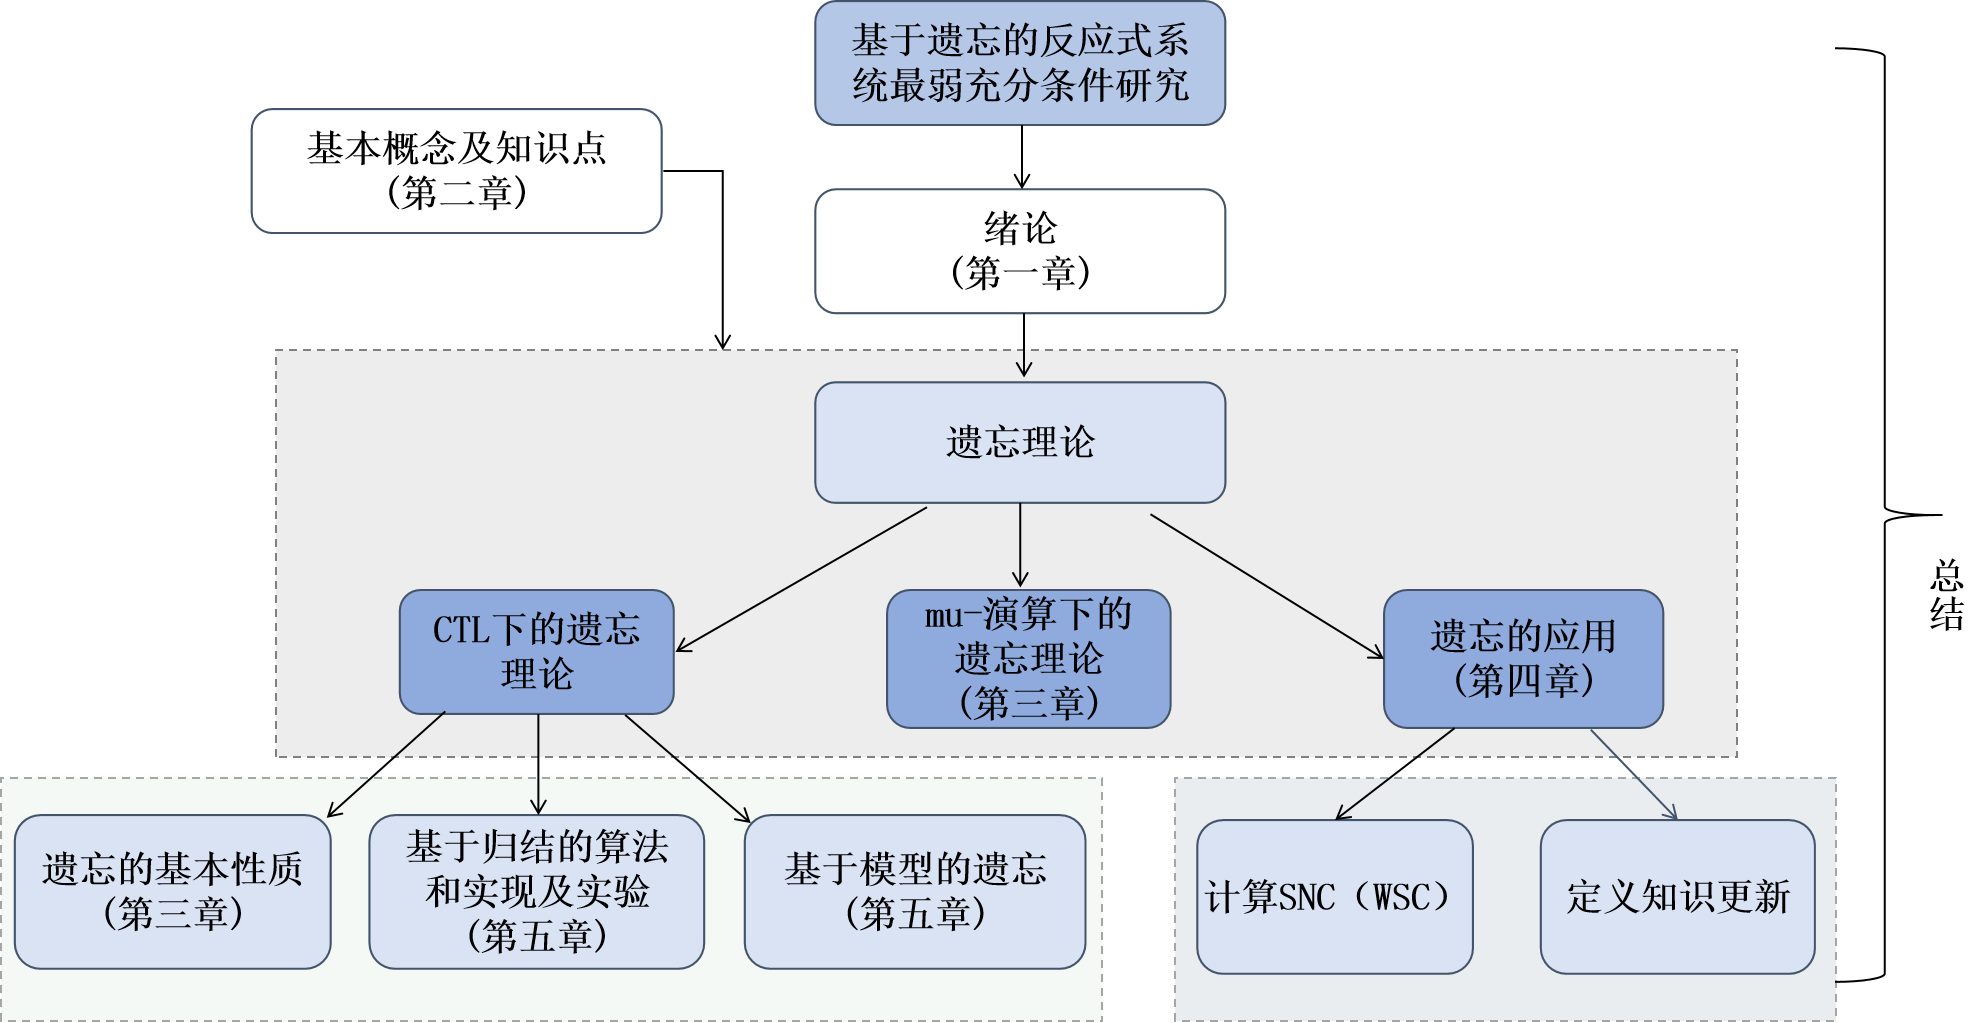
\includegraphics[width = 1\linewidth]{chapter01/zuzhi.png}
	\caption{本文的章节内容组织结构图}
	\label{fig:chapter1-research-structure}
\end{figure}

第\ref{chapter01}章为\textit{绪论},首先阐述了本文的研究背景及意义,并分析给出了存在的问题,凝练出本文研究需要解决的关键问题。基于上述分析,阐述了本文的研究内容和研究取得的主要成果。最后给出了本文的章节组织结构安排。


第\ref{chapter02}章为 {\em 背景知识},介绍了本文研究所涉及逻辑语言的语法语义及相关技术。首先,给出了经典命题逻辑下解释(赋值)的定义,以及相关语言的模型结构——Kripke结构。
然后,本章给出$\CTL$和$\mu$-演算的语法和语义。
最后,除了最强必要条件和最弱充分条件在经典逻辑和模态逻辑S5下的研究,本章还介绍了与上述逻辑语言密切相关的两个技术:遗忘和$\CTL$下的归结。



第\ref{chapter03}章 {\em 给出$\CTL$和$\mu$-演算遗忘的定义及其基本性质}。首先,给出一种新的互模拟定义,并介绍其基本属性;其次,使用互模拟来定义$\CTL$和$\mu$-演算下的遗忘,并研究遗忘的属性,包括表达性属性(representation theory)和复杂性结果等。本章指出$\CTL$遗忘是不封闭的,即存在某些公式的遗忘结果不能用$\CTL$来表示。此外,证明了$\mu$-句子遗忘的结果总是存在的,且不含有不动点操作的这类$\mu$-公式遗忘的结果总在这个类里面。

第\ref{chapter04}章 为{\em 遗忘理论在反应式系统中的应用}。讲述如何将遗忘应用于计算反应式系统在给定条件下的SNC(WSC)和定义知识更新。
此时,有限状态的反应式系统模型的WSC(SNC)可以通过遗忘来计算,且通过遗忘定义的知识更新满足Katsuno等人提出的八条基本准则。


第\ref{chapter05}章 为{\em $\CTL$遗忘的计算方法}。讲述了两种计算$\CTL$遗忘的方法:基于模型和基于归结的方法。此外,给出了基于归结的算法Prolog实现描述和实验结果分析。
在基于模型的计算$\CTL$遗忘中:第~\ref{chapter05:sec:model}节探讨了约束$\CTL$遗忘是封闭的情形;为此,提出了一种约束的互模拟,并定义给定深度的计算树在给定原子命题集下的特征公式,继而给出有限情况下Kripke结构在给定原子命题集下的特征公式;最后说明,在约束情形下,$\CTL$公式的遗忘结果总是$\CTL$公式可表达的。
在基于归结的计算$\CTL$遗忘中:首先,将$\CTL$公式转换为归结规则需要的子句形式——$\CTLsnf$子句;其次,使用归结规则计算要遗忘的原子命题上所有可能的归结结果;随后,移除那些含有要遗忘的原子命题的子句,并给出一种一般化的Ackermann引理消除一些新引入的原子命题;最后,将得到的结果转换成$\CTL$公式。此外,根据上述过程,提出计算$\CTL$遗忘的算法,并分析该算法的时间和空间复杂性。


%第\ref{chapter04}章 为{\em 基于归结的$\CTL$遗忘计算}。基于第\ref{chapter02}章的归结规则,本章探讨如何使用该归结系统计算$\CTL$下的遗忘。首先,将$\CTL$公式转换为归结规则需要的子句形式——$\CTLsnf$子句(后文详细介绍);其次,使用归结规则计算所有可能的需要遗忘的原子命题上的归结结果;随后,移除那些包含要遗忘的原子命题的子句,并给出一种一般化的Ackermann引理消除一些新引入的原子命题;最后,将得到的结果转换成$\CTL$公式。此外,基于上述过程提出计算$\CTL$下的遗忘的算法,并分析该算法的时间和空间复杂性。

%第\ref{chapter05}章 为{\em 约束$\CTL$下的遗忘}。在第\ref{chapter03}章所说,$\CTL$下的遗忘不是封闭的,因此在本章探讨了约束$\CTL$遗忘是封闭的情形。为此,本章提出了一种约束的互模拟,并给出给定深度的计算树在给定原子命题集合下的特征公式,继而给出有限情况下Kripke结构在给定原子命题集合下的特征公式。最后说明约束情形下$\CTL$公式的遗忘结果总是$\CTL$公式可表达的。




%第\ref{chapter06}章 为{\em $\mu$-演算下的遗忘}。$\mu$-演算是一种表达能力比$\CTL$强的时序逻辑,其具有均匀插值性质。本章给出$\mu$-演算下遗忘的定义和基本属性,包括模块性、交换性及同质性。此外,探讨了$\mu$-演算下的遗忘是封闭的,且对任意析取$\mu$-公式的遗忘可以在多项式时间内计算出来。
%最后,给出$\mu$-演算下关于遗忘算子的模型检测和推理问题的复杂性结果。



%第\ref{chapter07}章 为\textit{遗忘理论的应用}。讲述如何将遗忘应用于计算SNC(WSC)和定义知识更新。
%此时,有限状态的反应式系统模型的WSC(SNC)可以通过遗忘来计算,且通过遗忘定义的知识更新满足Katsuno等人提出的知识更新应该满足的基本准则。
%在这种情形下将公式的模型限制到有限状态空间,组成公式的原子命题也是有限的。经过

%第\ref{chapter08}章 为\textit{实验结果}。给出基于归结的算法实现模型的实验结果及分析。


第\ref{chapter09}章为\textit{总结与展望}。首先总结了本文的研究工作,进一步,展望了未来研究工作的方向和重点。
